
\documentclass[10pt,letterpaper]{article}
\usepackage[top=0.85in,left=0.85in,footskip=0.75in]{geometry}
% amsmath and amssymb packages, useful for mathematical formulas and symbols
\usepackage{amsmath,amssymb}
% Use adjustwidth environment to exceed column width (see example table in text)
\usepackage{changepage}
% Use Unicode characters when possible
\usepackage[utf8x]{inputenc}
% textcomp package and marvosym package for additional characters
\usepackage{textcomp,marvosym}
% cite package, to clean up citations in the main text. Do not remove.
\usepackage{cite}
% Use nameref to cite supporting information files (see Supporting Information section for more info)
\usepackage{nameref,hyperref}
% line numbers
%\usepackage[right]{lineno}

\usepackage{natbib}

\usepackage{graphicx}

\usepackage{float}

% color can be used to apply background shading to table cells only
\usepackage[table]{xcolor}

% array package and thick rules for tables
\usepackage{array}

\usepackage{dsfont}


%% END MACROS SECTION

\title{Triqler for Data Independent Aquisition Data}
\author{Patrick Truong \and Matthew The \and Lukas K\"{a}ll}


\begin{document}
%\linenumbers
\maketitle

\begin{abstract}
  %In this study we show that Triqler, a protein quantification and differential analysis tool based on probabilistical graphical models, has better performance than other protein quantification tools. To show this we compare different processing pipelines using different underlying concept for protein idenfication and quantification.
  
  In this study, we benchmark protein summarization methods for DIA data. A previous benchmarking attempt has shown that TOP3 generally resulted in lower variance and better quantification accuracy than built-in methods for DIA data. Since more sophisticated protein summarization methods have been shown to perform better for DDA data, there are reasons to believe that such methods would also work better for DIA data. Further, currently, there are is no evidence that protein summarization that worked well for DDA data would not work well for DIA data. In this study, we evaluate the performances of several protein summarization methods on DIA data. 
\end{abstract}
  

\section*{Introduction}
Label-free quantification (LFQ) using Mass spectrometry (MS) based proteomics is an effective method for studying the relative concentration of proteins in complex mixtures. Compared to Data-dependent acquisition (DDA), Data-independent acquisition (DIA) mass spectrometry allows for a broader dynamical range and more reproducible peptide detection 
 \cite{zhang2020DIA, Lu2021DIAmeter}. Stochastic and irreproducible precursor ion selection \cite{liu2004model} \cite{li2009database}, undersampling \cite{michalski2011more}, and long instrument cycle times \cite{li2009database} which has been problematic in DDA-methods are  addressed by DIA-methods such as such as SWATH-MS \{gillet2012targeted}, high-definition MS using alternating low and elevated energy acquisition in combination with ion-mobility separation (HDMS) \cite{geromanos2012using}, and all-ion fragmentation (AIF) \cite{geiger2010proteomics}. Computational methods for data processing, protein database searching, and statistical analysis of the quantitative methods all affect the final results. Evaluating such methods are therefore relevant \cite{gatto2016testing}. At the current state of DIA-proteomics objective benchmarking of the robustness and performance of the computational methods would greatly benefit quantitative proteomics \cite{navarro2016multicenter}. Previous efforts at DIA protein quantification benchmarking have indicated that the TOP3 method generally resulted in lower variance and better quantification accuracy than built-in methods \cite{navarro2016multicenter}. However, there are reasons to believe that more sophisticated methods would yield better protein quantification than TOP3-method. Simple summarization methods based on mean and median peptide intensity has been shown to produce unreliable protein abundance estimates \cite{goeminne2015summarization}, and more advanced summarization strategies for LFQ data has been proposed in literature \cite{silva2006absolute] \cite{cox2014accurate} \cite{zhang2018proteome} \cite{choi2014msstats}. In proteomics protein summarization methods such as Triqler\cite{The2018Integrated}, msStats \cite{choi2014msstats}, and msqrobsum \cite{sticker2020robust} has all been shown to perform better than TOP3 and there currently exists no reason why said methods would not theoretically be able to perform well for DIA-data. 
 
Protein quantification for DIA-proteomics could greatly benefit from having DDA protein quantification methods benchmarked for utilization for DIA data. To address this, we investigate the usage of DDA protein quantification method for performing protein quantification on DIA-data. Navarro et al. \cite{navarro2016multicenter} has previously constructed a high-quality data set for five widely used tools for analysis of SWATH-MS data (four peptide-centric query tools: OpenSWATH \cite{rost2014openswath}, SWATH 2.0, Skyline \cite{maclean2010skyline}, Spectronaut \cite{bruderer2015extending}, and one data-centric approach DIA-Umpire \cite{maclean2010skyline}). This is a good data set to perform benchmarking on protein summarization procedures because we have a reference point to compare against. Unbiased comparisons of software tools have been challenging for several reasons \cite{dufresne2014abrf}. Methods can be assessed by scientist lacking relevant expertise, the tested methods may be lacking sufficient documentation and the interpretation of test results may be subjective \cite{yates2012toward} \cite{leprevost2014best} \cite{pak2013clustering} \cite{faircomparison2015}. By using the same data set we can assure that the data set is processed consistently and further the analysis by extending it to protein summarization procedures.


\section*{Materials and methods}
\subsection*{Data description}

The data is a DIA dataset constructed by Navarro et al. benchmarking study \cite{navarro2016multicenter}. It is available from the ProteomeXchange Consortium with the dataset identifier PXD002952. The instrumentation used to process the data was TTOF6600 system with 32 fixed windows. In the repository, the data we use is referred to as the HYE124 hybrid proteome samples. It consists of tryptic peptides with the following ratios: Sample A composed of 65\% w/w, 30\% w/w yeast, and 5\% w/w E. coli proteins. Sample B was composed of 65\% w/w, 15\% w/w yeast, and 20\% w/w E. coli proteins. Further details about mass spectrometric instrumentation and data acquisition are available in Navarro et al. \cite{navarro2016multicenter}.    

\subsection*{General workflow}
In this study we investigate two DIA protein quantification workflows 1) DDA-based spectral library protein quantification (DDA-SLPQ) and 2) Pseudo spectra-based spectral library protein quantification (PS-SLPQ). The DDA-SLPQ workflow uses MSFragger to perform a DDA-search and EasyPQP to construct a spectra library from the DDA-search results. OpenSwath Workflow is then used with a spectral library to perform an analysis on the DIA data. PyProphet is used for statistical validation and TRIC is used for feature alignment before protein quantification using Top3, MSstats, and msqrobsum (TRIC is not used for triqler protein quantification). The PS-SLPQ workflow is conducted using fragpipe software. It uses DIA-Umpire signal extraction to extract pseudo-spectra from the DIA data. The pseudo-spectra is searched using conventional DDA-search using MSFragger and the spectral library is build using easyPQP. The DIA-data is quantified with DIA-NN using the pseudo-spectra-based spectral libraries. The DIA-NN uses a mProphet-based algorithm for statistical validation \cite{reiter2011mprophet} \cite{demichev2020dia}. 

(add a third later encyclopedia) 

(add workflow schematics )

\subsection*{Data preparation and spectral library generation}
The .wiff files are converted to .mzML files in a centroided format using msconvert (using windows OS msconvert version X.X) with the following options: [check options]. 

Two approaches were used for spectra library generation: DDA acquisition-based spectral library generation and Prosit-based spectral library generation using only .fasta file \cite{searle2020generating}. 

DDA acquisitions of samples from each species (human, yeast, E. coli) were provided in triplicates for spectral library generation. Uniprot FASTA files with one protein sequence per gene were concatenated for each species (UP000005640, UP000000625, and UP000002311, acquired on 2021-06-16).To control for the effect of different protein inference strategies (protein group, parsimony, etc.) a modified .fasta file, without shared peptides, was used for database search. The unfiltered FASTA files contained 20 590 human proteins, 6 046 yeast proteins, and 4 373 E. coli proteins. After filtering the FASTA file contained 20 302 proteins (-288 human proteins), 5 848 yeast proteins (198 yeast proteins), and 4 306 E. Coli proteins (-67 E. Coli proteins). Each sequence with length $>$7 amino acids mapping only to one protein. The FASTA file contained reverse sequences as decoys for target-decoy analysis. MSFragger with parameters: [check parameters] was used for DDA-search, statistical validation was performed by peptide prophet and protein prophet, and EasyPQP with parameters: [check parameters] was used for the spectral library building. OpenSwathDecoyGenerator was used with default settings to generate decoys for the resulting spectral libraries.  

For Prosit-based spectral library generation, the FASTA file was converted to Prosit input format using encyclopeDIA converter. Prosit\_2020\_intensity\_cid model was used as an intensity prediction model and Prosit\_2019\_irt was used as iRT prediction model.  


\subsection*{Protein inference problem and reduced database}

In bottom-up proteomics, redundancy in the matching of peptides to proteins hits is a challenge \cite{nesvizhskii2005interpretation}. The Parsimony principle reports the minimum set of proteins which include all the observed peptides (Occam's razor principle), thereby resolving shared and ambiguous evidence. This method typically reduces the size of the protein list where peptides could belong to several proteins, as the cost of losing potential protein identifications. In addition, it may also lower the reproducibility of the identified proteins\cite{serang2012recognizing}. While the protein grouping approaches bunch together proteins based on different schemas. For example, it is possible to group proteins that map to identical peptides, or when proteins contain overlapping subsets of peptides. The protein groupings are often assigned post peptide identification, which is contrary to good statistical practices to formulate the hypothesis before data are observed \cite{serang2012recognizing}. An example of parsimony and protein grouping is shown in \textbf{table 1}. 


\begin{table}[!htbp]
\begin{tabular}{llllllll}
          & Peptides &   &   &   &   & Parsimony reported & Grouping reported \\
          & 1        & 2 & 3 & 4 & 5 &                    &                   \\
Protein A & x        & x &   &   &   & Yes                & Yes               \\
Protein B &          & x & x &   &   & No                 & Yes               \\
Protein C &          &   & x & x &   & Yes                & Yes              	
\end{tabular}
\newline
\textbf{Table 1:} Example of Parsimony reported and protein grouping reported proteins.
\end{table}

In this benchmarking study, we remove proteins with shared peptides. Using different methods for protein inference yields a different amount of protein matches given the same amount of observed peptides. Ideally, the number of proteins compared between different protein quantitation methods should be the same when benchmarking. By removing proteins with shared peptides from the FASTA database the protein inferences procedures will yield the same protein identifications. This should give a fair comparison regardless of the protein inference method used in the different protein quantitation pipelines.

\subsection*{DIA methods}
Write about why different methods where used.

\subsubsection*{OpenSwath Analysis}
Version (version) of OpenSwath was used. The spectral library generated above is converted to .pqp format using TargetedFileConverter. Data analysis was conducted using OpenSwathWorkflow with parameters (-Scoring:TransitionGroupPicker:background\_subtraction original -Scoring:stop\_report\_after\_feature -1, -min\_upper\_edge\_dist 1, -tr\_irt hroest\_DIA\_iRT.TraML, -extra\_rt\_extraction\_window 100, -min\_rsq 0.95, -min\_coverage 0.6, -Scoring:Scores:use\_dia\_scores true, -rt\_extraction\_window 600, -mz\_extraction\_window 30, -threads 10, -Scoring:DIAScoring:dia\_extraction\_unit ppm). After data extraction the data .osw output was merged using pyprophet merge option and pyprophet was used for statistical validation. Pyprophet export was used without FDR filtering (--max\_global\_protein\_qvalue 1.0, --max\_global\_peptide\_qvalue 1.0, --max\_rs\_peakgroup\_qvalue 1.0, --max\_transition\_pep 1.0) to give a complete list of peptide quantifications for further down-stream analysis.

\subsubsection*{DIAUmpire and DIA-NN analysis}
DIAUmpire signal extraction (SE) was used through Fragpipe GUI (v15.0). Default parameters was set (MS1 PPM: 10, MS2 PPM: 20, Max Missed Scans:1, Mass Defect Filter On, RP max: 25, RF max: 500, Corr Treshold:0, Delta Apex: 0.2, RT Overlap 0.3, Mass Defect Offset 0.1, Isotope Pattern: 0.3, MS1 SN: 1.1, MS2 SN 1.1, Adjust fragment intensity On). MSFragger was used on the resulting .mzML files from DIAUmpire SE with default parameters for Peak Matching (PPM: [-20, 20], Fragment mass tolerance PPM: 20, Calibration and Optimization: Mass Calibration, Parameter optimization, Isotop error: 0/1, Data type: DDA, ), protein digestion (Load rules: stricttrypsin, Enzyme name: stricttrypsin, Cut after: KR, Cleavage: ENZYMATIC, Missed cleavages: 2, Clip N-term M: On, Peptide length 7-50, Peptide mass range: 500-5000, Split database: 1) and Modification (Variable modifications: M, \/[\^, Fixed modification: "all selected"). 

\subsubsection*{EncyclopeDIA and PECAN analysis}
Prosit was used to construct spectra libraries from the modified FASTA files. The fragmentation model used was "Prosit - Model - Fragmentation" and the iRT model "Prosit - Model - iRT" (available from https://figshare.com/projects/Prosit/35582).
...

\subsection*{Protein quantification methods}

\subsubsection*{Triqler}

Triqler is based on probabilistic graphical models that allow error information to propagate through all steps from MS1 feature detection to protein quantification. Unconventionally, it produces posterior probabilities for fold changes rather than point estimates \cite{The2018Integrated}. The robustness of results when faulty imputation of missing data is conducted is a common problem in missing data analysis \cite{ma2018bayesian}. These posteriors incorporate information about uncertainty and therefore should result in robust protein quantification. Triqler has been shown to distinguish more proteins for DDA data compared to other DDA protein quantification methods. \cite{The2018Integrated}. 

Triqler was used with --fold\_change\_eval between 0-2 with 0.04 increments. It computes the two-sided differential probability threshold between the two samples given a fold change evaluation limit. 

\subsubsection*{Top3}
The precursors are filtered by q-value \textgreater 1\% and the average of the three largest peptide intensities are taken for each protein. Protein with only one detected peptide (single hit proteins) and proteins detected only in two injections are discarded.

\subsubsection*{MSstat}
 MSstats customizes a linear mixed model to the specific experiment and each protein \cxite{choi2014msstats}. SWATH2Stats was used to convert the .osw output files to MSStats input format. dataProcess function in the MSstats package is used for data pre-processing and quality control of the MS runs of the data into quantitative data for model fitting and group comparison (Default parameters was used (specifically the peptide-level data is filtered by an m-score < 0.01 to reduce the memory consumption before running MSstats). quantification function in the MSstats package is applied on the pre-processed data to generate the quantification results for each protein.  

\subsubsection*{Msqrobsum}
Msqrobsum provides protein summarization that account for peptide specific effect (MSqRob inference framework \cite{goeminne2020msqrob}) and are further processed using robust ridge regression. The MSqRob inference frame work is a linea regression peptide-based mixed model. The parameters for the model are tuned using penalised estimation and multiple-testing is corrected using Benjamini-Hochberg FDR procedure. 

The data is processed according to default setting. It preprocessed using MSnBase R/Bioconductor package \cite{gatto2012msnbase} and normalized using Variance Stabilizing Normalization \cite{von2002variance}. 


%(Note: write something about difference FDR computation method and conservativeness, and why it does not make sense to compare between processing method, but it is ok to compare between post-processing methods)



\subsection*{Benchmarking methods}

\subsubsection*{Variance Structure - why the DDA methods works and makes sense}
The field of protein quantification is relatively new. Many protein quantification methods have been developed for LFQ data and performance has been established on DDA data. Many of these methods should be generalizable for DIA data. Triqler (probabilistic graphical model), MsStats (linear mixed model) and MSqRob (Ridge Regression) all require a homoskedastic variance. This is investigated using statistical visualization of the data.

\subsubsection*{Protein level results - scatter plot}

\subsubsection*{Differential abundance - log2distribution and number of differentially expressed proteins}
The differential expressed proteins are proteins with a log2-fold change of proteins with a q-value lower than a certain threshold for q-value based protein summarization methods (Top3, msStats and msqrob), while triqler computes a posterior distribution based  log2-fold change. 

(Write formula for triqler)
(Write formula for other methods)

\subsubsection*{FDR control (calibration plot)}
An FDR control of the quantification methods is required for benchmarking. We use the False Discovery Proportion (FDP) and True Positive Rate (TPR). FDP is calculated using and calculated using 

	\[FDP = \frac{ \text{false positives}}{\text{true positive} + \text{false positive}}

and,

	\[TPR = \frac{\text{true positives}}{\text{all positives}}


The FDP is calculated using the fraction of human proteins discovered as DE and the TP is the fraction of E.Coli and Yeast discovered. 



\section*{Results}

\subsection*{Variance structure}
(Write why different protein quantification methods and why triqler should be better in theory.) 

 In fig. \ref{fig:variance_to_mean_ratio} it is shown that the variance-to-mean intensity ratio does not increase for larger means. As the variance does not increase with mean heteroskedasticity does not exist in the DIA-data. This implied that methods based on linear regression, linear mixed models and other models requiring stable variance structure could be used for DIA protein quantification.

  %(Write something about implication of this)
  %(I COULD TRY TO SHOW THIS WITH QQ PLOT INSTEAD). 

\begin{figure}[H]
    \centering
    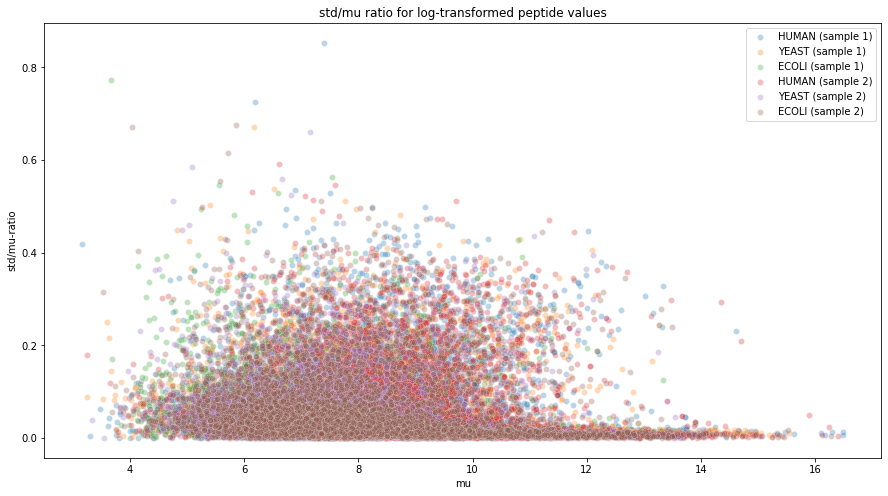
\includegraphics[width=12cm]{../../result/2021-08-13_docs_plots/variance_to_mean_plot.png}
    \caption{mean vs. variance-to-mean ratios. The variance-to-mean ratios stays similar across the means.}
    \label{fig:variance_to_mean_ratio}
\end{figure}



\subsection*{Protein quantification}

Log-transformed ratios (log2(A//B)) of proteins (humans proteins in orange, yeast proteins in green, and E. Coli proteins in blue) were plotted for each benchmarked software over the log-transformed intensity of sample A. The dashed horizontal line represents the expected log-fold change, while the fitted dashed line represents a linear regression for each species. Fig. \ref{fig:OSW_scatter} shows the results for OpenSwath and fig. \ref{fig:OSW_scatter} shows the results for DIA-NN. TOP3 and MsStat gives least biased results as protein intensities gets higher. Triqler gives the most biased results. 

\begin{figure}[H]
    \centering
    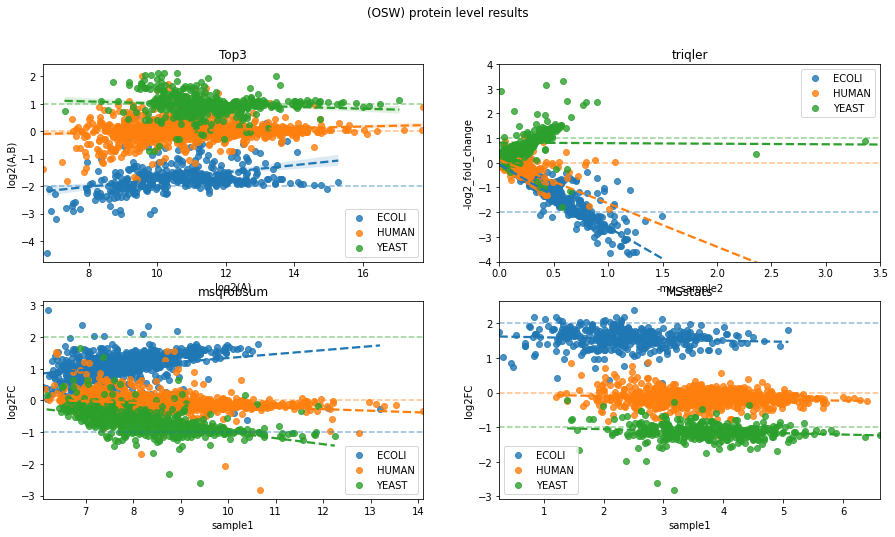
\includegraphics[width=16cm]{../../result/2021-08-13_docs_plots/OSW_protein_level_benchmark_scatter.png}
    \caption{OSW Protein level results from Triqler, Top3, MSstats and MSqRobSum.}
    \label{fig:OSW_scatter}
\end{figure}

\begin{figure}[H]
    \centering
    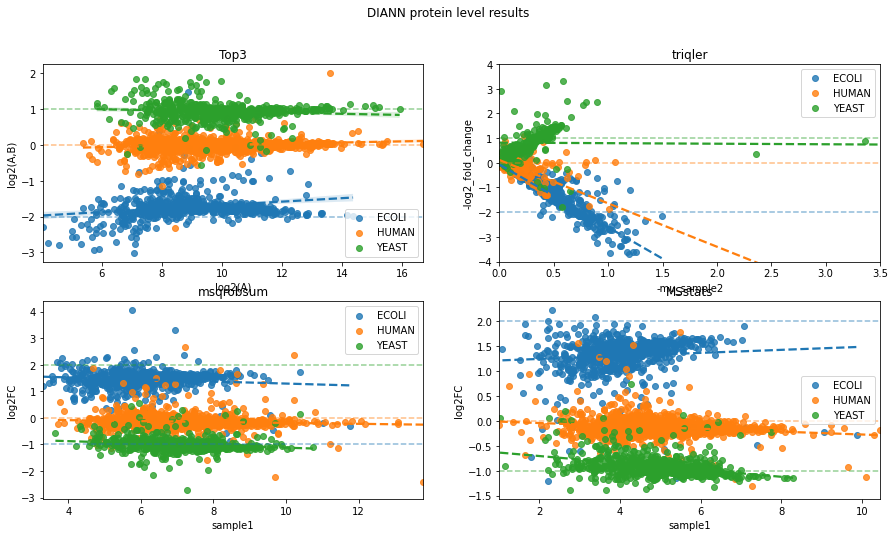
\includegraphics[width=16cm]{../../result/2021-08-13_docs_plots/DIANN_protein_level_benchmark_scatter.png}
    \caption{DIANN Protein level results from Triqler, Top3, MSstats and MSqRobSum.}
    \label{fig:OSW_scatter}
\end{figure}

Fig. \ref{fig:intensity_distribution} and \ref{fig:DIANN_intensity_distribution} show the protein quantity distributions with the different species; human (orange), E. Coli (blue), and yeast (green) highlighted in different colors for OSW \ref{fig:intensity_distribution} and DIA-NN \ref{fig:DIANN_intensity_distribution}. The human and yeast distribution apex is not centered at 0 in MsStats and MSqRob, while it is centered for triqler and top3. Likewise, the distribution for e.coli is closer to the true log2 fold change ratios for triqler and top3, while the apexes are skewed towards 0 for MsStats and MSqRob for both OSW and DIA-NN.     

\begin{figure}[H]
    \centering
    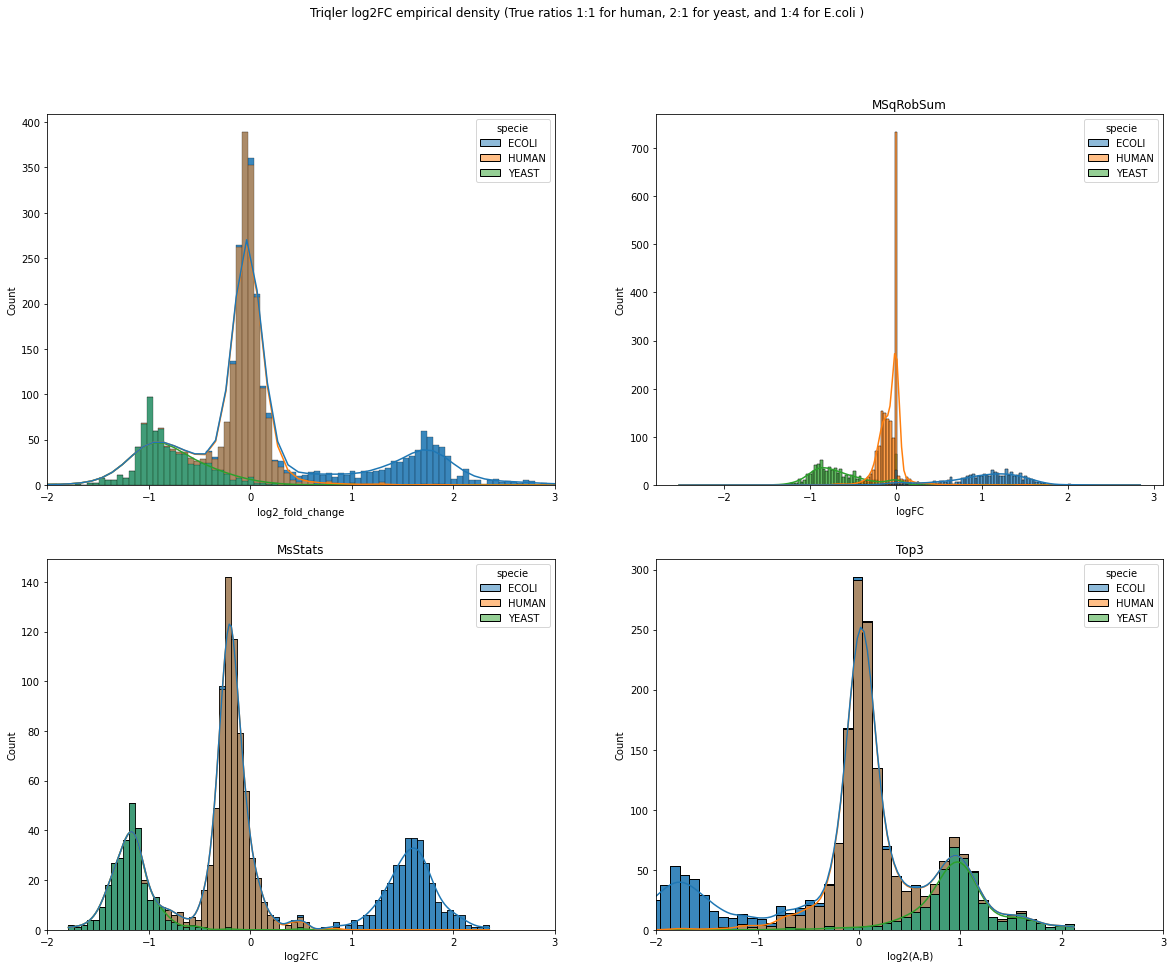
\includegraphics[width=16cm]{../../result/2021-08-13_docs_plots/intensity_plot.png}
    \caption{OSW Protein quantity distributions from Triqler, Top3, MSstats and MSqRobSum.}
    \label{fig:intensity_distribution}
\end{figure}

\begin{figure}[H]
    \centering
    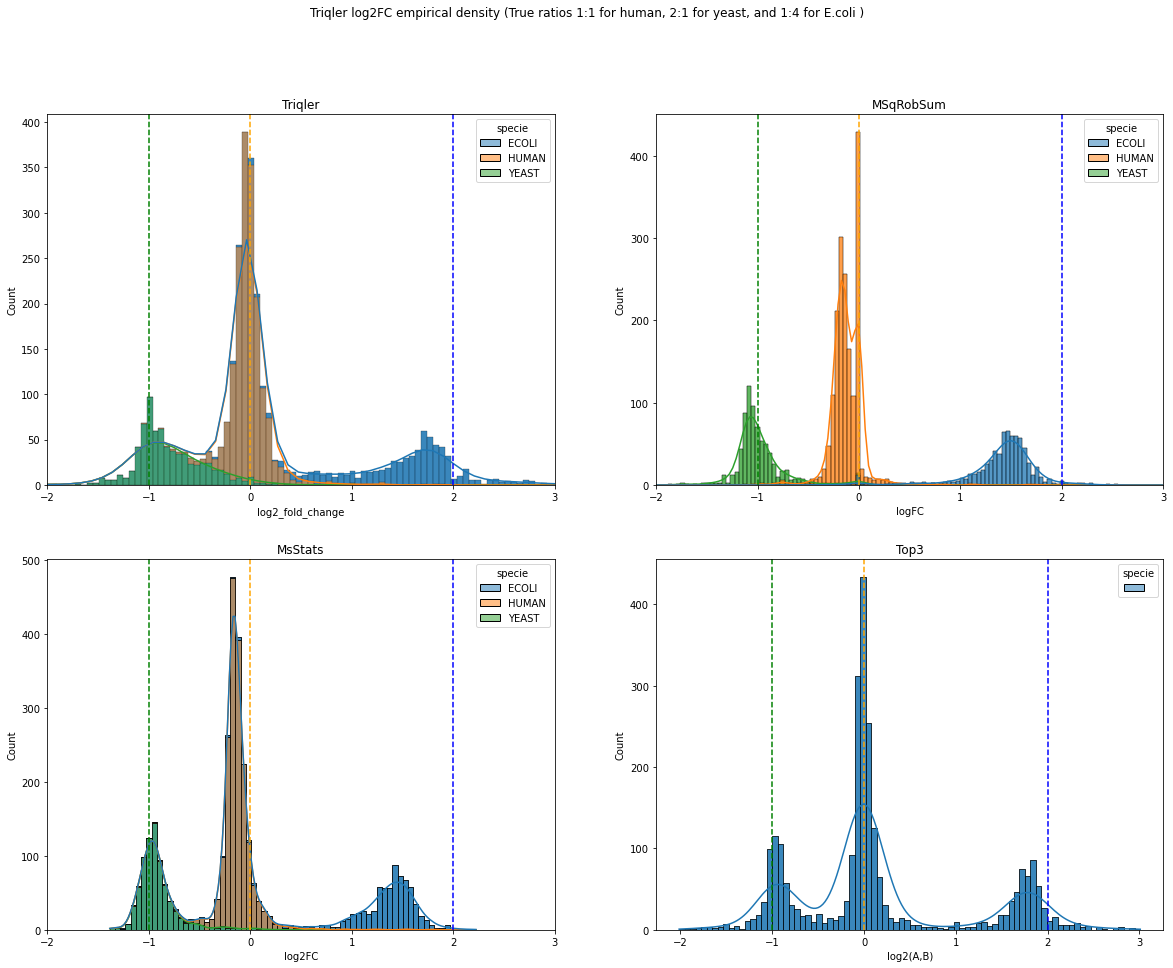
\includegraphics[width=16cm]{../../result/2021-08-13_docs_plots/DIANN_intensity_plot.png}
    \caption{DIANN Protein quantity distributions from Triqler, Top3, MSstats and MSqRobSum.}
    \label{fig:DIANN_intensity_distribution}
\end{figure}


Fig. \ref{fig:osw_n_diff_exp} and \ref{fig:DIANN_n_diff_exp} shows that the number of differentially expressed proteins is significantly higher for Triqler and MSqRobSum at different false discovery rates. MSqRobSum has a slightly higher number of differentially expressed proteins than triqler for OSW, and Triqler has slightly higher number of differentially expressed proteins for DIA-NN. The difference between the number of differentially expressed proteins are also smaller for MsStats and triqler and MSqRobSum for DIA-NN. 

\begin{figure}[H]
    \centering
    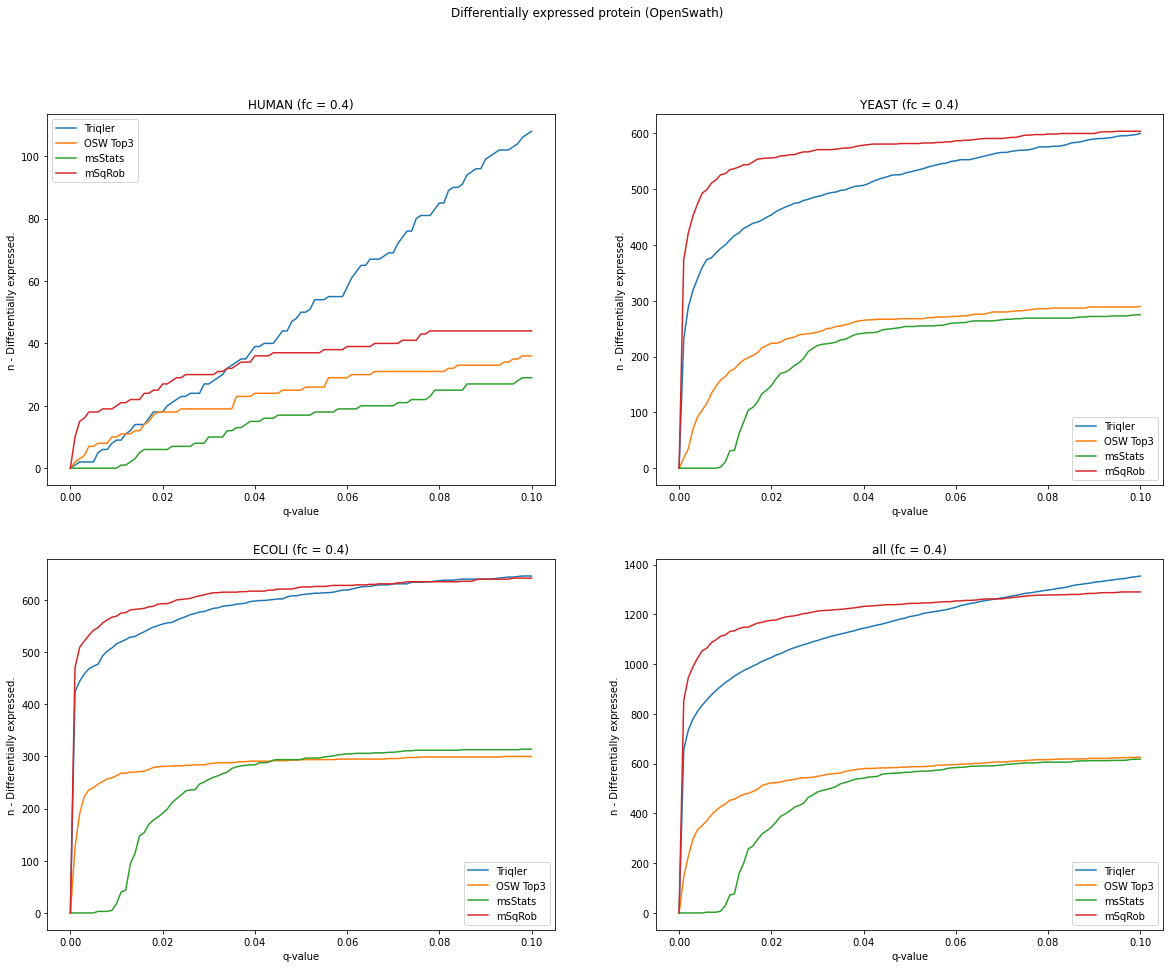
\includegraphics[width=16cm]{../../result/2021-08-13_docs_plots/n_diff_expressed.png}
    \caption{OSW Number of differentially expressed proteins for an OpenSwath analysis with triqler, top3, MsStats and MSqRobSum protein summarization.}
    \label{fig:osw_n_diff_exp}
\end{figure}

\begin{figure}[H]
    \centering
    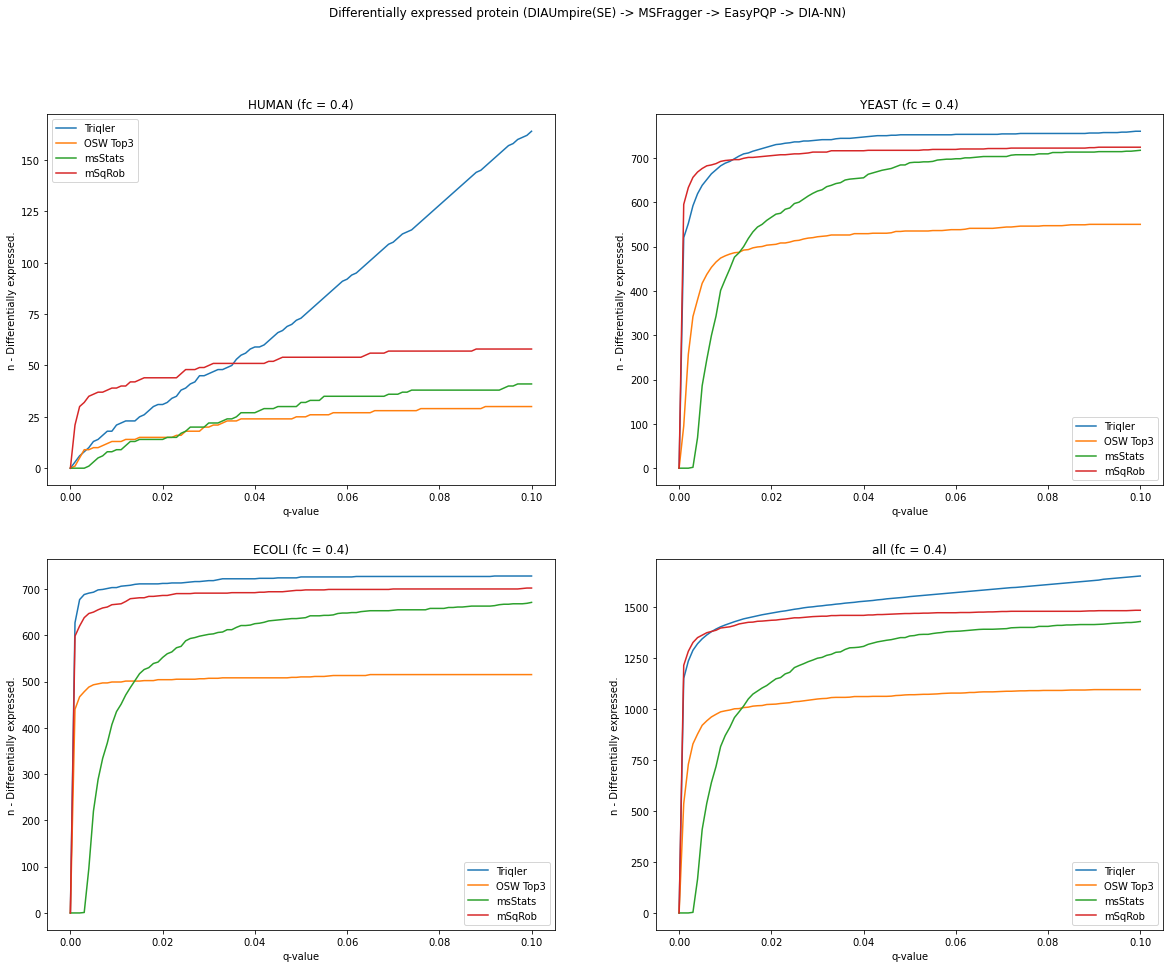
\includegraphics[width=16cm]{../../result/2021-08-13_docs_plots/DIANN_n_diff_expressed.png}
    \caption{DIANN Number of differentially expressed proteins for an OpenSwath analysis with triqler, top3, MsStats and MSqRobSum protein summarization.}
    \label{fig:DIANN_n_diff_exp}
\end{figure}



Fig. \ref{fig:osw_n_diff_exp} and \ref{fig:DIANN_n_diff_exp} shows that the ratio of false positives (human proteins) to the number of differentially expressed proteins for a given q-value level is more linear for triqler. At log2FC = 2 all methods are conservative at low q-values and anti-conservative at higher q-values. Triqler is better calibrated for low q-values and gets more conservative as the q-value threshold is increased. Top3, MsStats, and MSqRob are more conservative at low q-values and get less conservative as the q-value threshold increases.  

   
\begin{figure}[H]
    \centering
    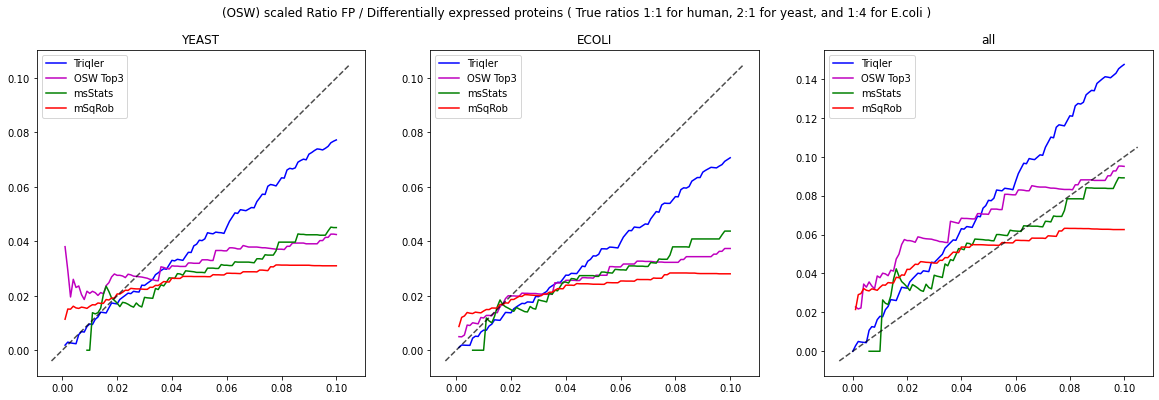
\includegraphics[width=16cm]{../../result/2021-08-13_docs_plots/calibration_plot_scaled.png}
    \caption{OSW Q-value (x-axis) and false positive / number differentially expressed protein (y-axis) ratio.}
    \label{fig:osw_n_diff_exp}
\end{figure}

\begin{figure}[H]
    \centering
    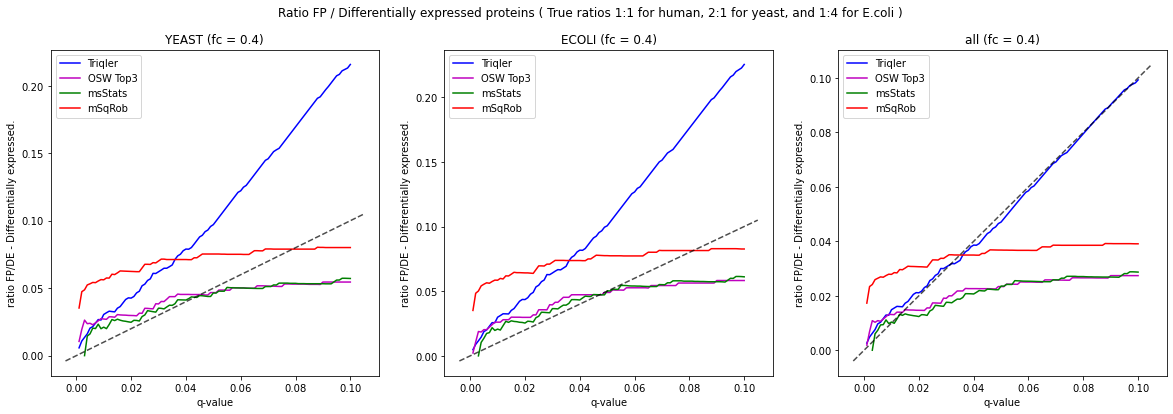
\includegraphics[width=16cm]{../../result/2021-08-13_docs_plots/DIANN_calibration_plot.png}
    \caption{DIANN Q-value (x-axis) and false positive / number differentially expressed protein (y-axis) ratio.}
    \label{fig:DIANN_n_diff_exp}
\end{figure}



\begin{figure}[H]
    \centering
    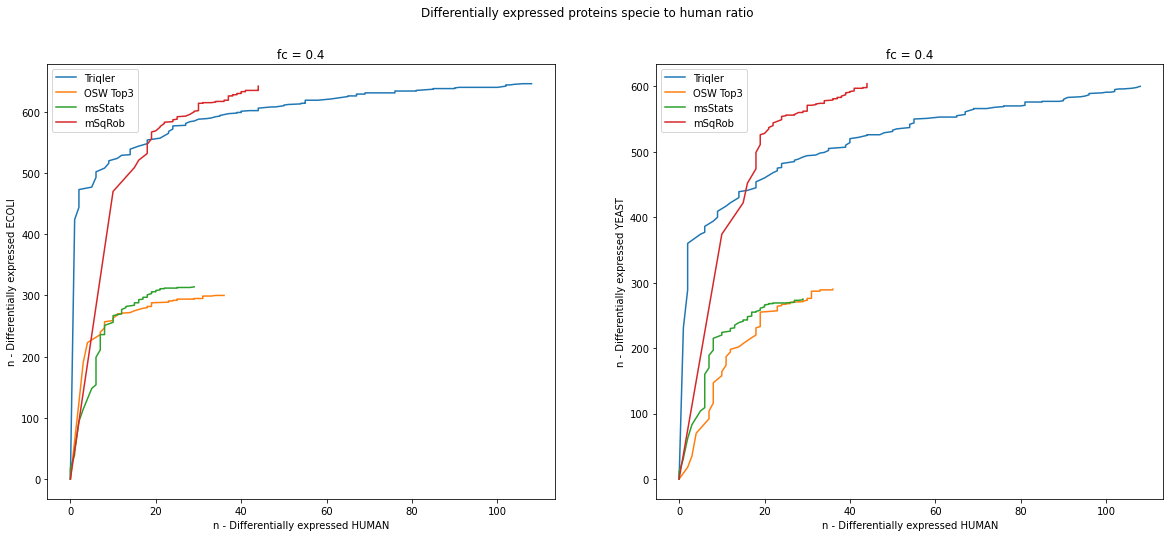
\includegraphics[width=12cm]{../../result/2021-08-13_docs_plots/de_human_vs_de_specie.png}
    \caption{OSW Number of differentially expressed humans (x-axis) and differentially expressed e.coli and yeast (y-axis).}
    \label{fig:osw_n_diff_exp}
\end{figure}

\begin{figure}[H]
    \centering
    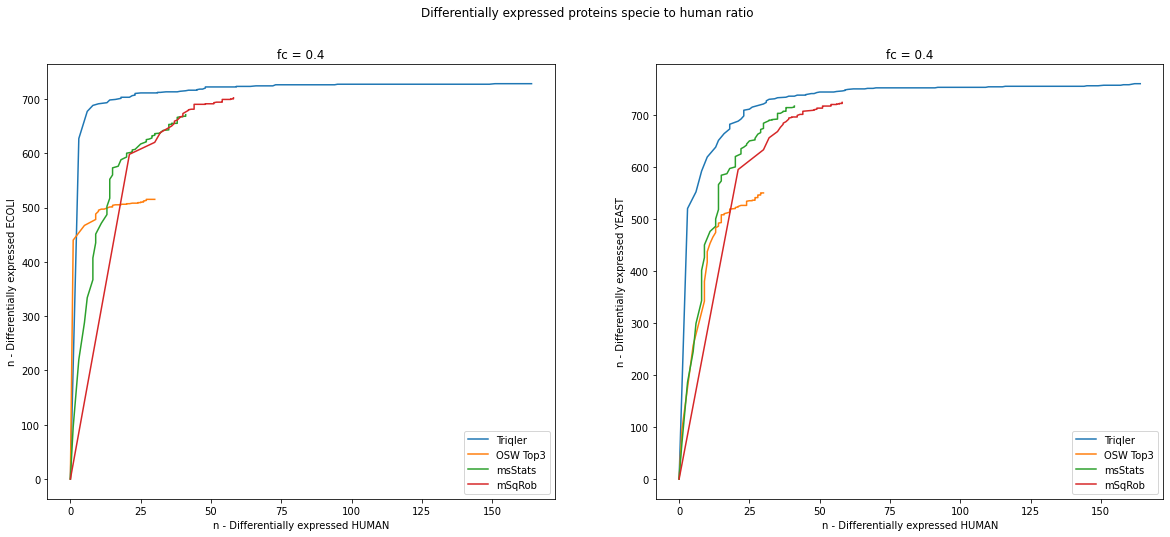
\includegraphics[width=12cm]{../../result/2021-08-13_docs_plots/DIANN_de_human_vs_de_specie.png}
    \caption{DIANN Number of differentially expressed humans (x-axis) and differentially expressed e.coli and yeast (y-axis).}
    \label{fig:osw_n_diff_exp}
\end{figure}

\section*{Discussion}

\section*{Acknowledgements}


\section*{Funding}

This work has been supported by a grant from the Swedish Foundation for Strategic Research (BD15-0043).

\section*{Supporting information}

\bibliographystyle{plain}
%\bibliography{benchmark}
\bibliography{benchmark.bib}
\end{document}

